\chapter{Evaluation}\label{chapter:evaluation}

% !TeX root = ../main.tex
% Add the above to each chapter to make compiling the PDF easier in some editors.
%\chapter{Case study}\label{chapter:EA documentation in an insurance company} 
% IST-Analyse
% EA documentation in an insurance company

The first section of this chapter introduces the methodology of the case study. 
%The case study design is a research methodology the evaluation of the implemented prototype in a case study.
The second section will explain the challenges that influence the IT landscape of the insurance company. These are divided into internal and external challenges. In the next section~\ref{section:asislandscape} the current IT landscape of the enterprise is described. In addition to the as-is IT landscape, the current process of the EA documentation in the insurance company was analyzed during this master-thesis. 
In the following section~\ref{section:targetitlandscape} the target IT landscape will be described.
In section~\ref{section:derivedrequirements}, the derived requirements to automate the EAD process will be presented.
At the end of this chapter the prototype is evaluated.

\section{Case Study Design}\label{section:casestudy}

The case study was conducted according to the research methodology for software engineering from Per Runeson. \cite{Runeson2009}

\subsection{Case study objectives}\label{subsection:casestudyobjectives}

This case will identify the current practice and the challenges regarding the EAD process in a german insurance company. The case study evaluated the suggested solution of an automated EAD process and its prototype derived from the requirements found out during the literature research. To improve the solution the prototype was evaluated in the company to derive further requirements for an automated EAD.

\subsection{Case study definition}\label{subsection:casestudyobjectives}

The subject of this case study is an international insurance company located in Germany. The investigation in this case will mainly focus on the Enterprise Architecture Documentation process within the company. To understand the process, the study will take a look at the IT landscape to retrieve information how the EA relevant components interact with each other and what challenges influence the IT landscape. This will give an overview to find out why the enterprise is documenting EA relevant information in that way.
%Darf ich das schreiben: MAtheus fragen
%1000 entwickler
%2000 applikationen, daovn 400 in 2 clouds
The following numbers give a brief overview of the complexity of the enterprise. The IT landscape of the enterprise consists approximately of 2000 applications, 400 running on cloud based environments and the enterprise has nearly 1000 developers.

\subsection{Case study methodology}\label{subsection:casestudymethodology}

\subsubsection{Research questions -  what to know?}
%How  to  assign  the  application  landscape  to  business  domains?
%How  to  obtain  EA  relevant  information  from  the  runtime  behaviour  ofcloud-based environments?
%How to automate the assignment process with an integrated toolchain?
%How  does  a  prototype  implementation  of  the  automated  documentationprocess of cloud applications look like?
The research questions that are going to be answered are mentioned in ~\ref{section:researchquestions}.
RQ1, RQ2 and RQ3 are relevant for the case study. The aim is to see if the questions can be answered during the case study and the prototype evaluation to improve the automated EAD.

\subsubsection{Methods — how to collect data?}

As mentioned by Runeson et al. \cite{Runeson2009} the following information sources can be used to collect data:

\begin{itemize}
    \item Different data sources
    \item Archival data
    \item Interviews
\end{itemize}

%Archival data refers to, for example, meeting minutes, documents from different development phases, organizational charts, financial records, and previously collected measurements in an organization

During the case study a literature research was conducted to derive challenges and requirements from literature to be able to compare the information to the current situation of the company.

An analysis of the archived data of the company was executed during the thesis in order to gain more knowledge about the IT landscape, the reasons of the current documentation process, challenges changing the landscape and what the enterprise expects to be improved or even automated.

To retrieve more information informal and semi-structured interviews were conducted. The interviews were divided into 2 parts. The first part explained the motivation and the objectives of the thesis. The motivation introduced a brief overview of the scope of the thesis and the objectives includes the research questions to be answered. The second part of the interviews consisted of questions regarding the findings during the research of the current situation.

\section{Challenges influencing the IT landscape}\label{section:influencingfactors}

This section will describe the influencing challenges that have an impact on the IT landscape of the german insurance company. To understand the IT landscape an overview of the main influencing challenges is presented. First, the external ones such as regulations are explained. Secondly, the internal challenges are be mentioned. Finally, the EAD process will be described. 

\subsection{External challenges}\label{subsection:externalinfluencingfactors}

The section will describe the most important external challenges that change the IT landscape of the enterprise and thus have an impact on the EAD. There are three regulations that mainly influence the EAM. The first regulation is the General Data Protection Regulation (GDPR). The second factor affecting the IT landscape is the VAIT Regulation. The last regulation influencing the IT landscape is the international standard ISO 22301.

\subsubsection{General Data Protection Regulation}

The General Data Protection Regulation\footnote{\url{https://eugdpr.org/}} (GDPR) is a European Data Protection Regulation that enforces all member states of the European Union to harmonize data privacy laws. The GDPR is related to the processing of personal data. It assures fundamental rights of  persons, especially the right to the protection of personal data. GDPR enforces the enterprises to know exactly which information systems store personal data and how this information systems can be secured to protect the personal data from external hazards. An inventory of information systems related to the processing and storing of personal data is therefore required. This regulation demands a transparent and complete documentation of the IT landscape.

\subsubsection{VAIT Regulation}

The regulation "Versicherungsaufsichtliche Anforderungen an die IT" (engl. "Insurance supervisory requirements for IT") (VAIT) affects the IT of insurance companies with headquarters in Germany. The use of IT in companies, including IT services offered by IT service providers, is of central importance to insurance companies. The circular letter published in the context of the regulation mentioned contains information on the interpretation of the regulations on business organization in the Insurance Supervision Act  (in german "Versicherungsaufsichtsgesetz") (VAG) insofar as they relate to the technical organizational equipment of the companies. It makes these regulations binding for Federal Financial Supervisory Authority (in german "Bundesanstalt für Finanzdienstleistungsaufsicht") (BaFin), thereby ensuring consistent application to all companies and groups. The circular letter provides a flexible and practical framework, in particular for the management of IT resources, information risk management and information security management. \cite{Anforderungen2018}

The main requirement affecting the EAD is the IT operations requirement. The IT operation must implement the fulfillment of the requirements resulting from the implementation of the business strategy as well as the IT-supported business processes. The components of the IT systems and their relationships to each other should be managed appropriately and the inventory information collected should be updated regularly and on an ad hoc basis. The stock information includes in particular: Inventory and purpose of the components of the IT systems with the relevant configuration information, location of the components of the IT systems, compilation of the relevant information on warranties and other support contracts (possibly linking), information on the expiration date of the support period of the components of the IT systems, accepted Period of unavailability of the IT systems and the maximum tolerable data loss. \cite{Anforderungen2018}

\subsubsection{ISO 22301}

The ISO 22301\footnote{\url{https://www.iso.org/}} standard represents the latest international policy for Business Continuity Management (BCM) and was released in 2012. Its objective is to assist in the reduction of business interruptions due to unforeseen emergencies. This norm is an update of the standards ISO 31000 and ISO 27001. It is considered a universal standard in the sense that they apply to companies of all sizes and regardless of the used technologies.

To ensure the reduction of unforeseen emergencies an IT emergency system should be introduced to act as a a holistic management system. That includes monitoring and regular review of the IT landscape. These two aspects enable one of the main components of the standard execution: the Business Impact Analysis. 

The Business Impact Analysis (BIA) is a complex task that includes important corporate resources as a precautionary measure: specialists, executives and corporate management. The analysis includes the collection and identification of processes and functions,
the required resources such as staff, but also hardware resources like IT facilities, buildings, warehouses with their technical equipment. The analysis also include dependencies on IT processes, the definition of the core processes and impacts and recovery times. \cite{Osterhage2016}

\subsection{Internal challenges}\label{subsection:internalinfluencingfactors}

The internal challenges presented in the following paragraphs are mainly the drivers that have an impact on the IT landscape of the enterprise.

\subsubsection{Main business system}

The main business system of the insurance company has developed over time into a monolithic system. System components were built to connect new systems or applications to enable a communication between those. The added layers, components and adapters led to an not transparent and not maintainable monolithic system. The system contains several business logical aspects which results as an additional challenge for documenting the EA. To improve the transparency of the monolithic architecture the enterprise decomposed the system into modules to gain information about the dependencies to other applications and/or systems. 

\subsubsection{Business Continuity Management}

Driven by the ISO standard 22301 the german insurance company of this case study is also obliged to fulfill this regulation through a BCM project. The company is exposed to increasing risks that endanger the continuous and timely provision of its services to the customer. 
%Contributing to this are various developments and trends in society and the economy, such as growing globalization, increasing networking, centralization, automation, outsourcing.
Due to the increasing complexity of business processes, their increasing dependence on information technology and external service providers, external events such as fire, flood, the failure of information technology or external service providers can have a major impact.

The Business Continuity Management (BCM) is a management process with the aim of early identification of serious risks for the enterprise, which endanger the existence of the enterprise, and to establish measures against them. In order to ensure the viability and thus the existence of the company, appropriate preventive measures must be taken, which on the one hand increase the robustness and reliability of the business processes and on the other hand enable rapid and targeted response in an emergency or crisis.

The goal of the BCM is to ensure that important business processes are not or only temporarily interrupted, even in critical situations, and that the economic existence of the enterprise remains secured even in the event of a major loss event. A holistic view is therefore crucial. To consider are all aspects that are required to continue critical business processes when a claim event occurs, not just the Information Technology resource. IT emergency management is part of the BCM.
Critical business processes in the sense of emergency management means "time-critical", so that this process requires a faster resumption of activity, otherwise a high level of damage can be expected. The high damage can result from financial losses, violations of laws or contracts, from image damage or other damage scenarios.
A business process classified as "uncritical" does not mean that it is unimportant to the enterprise, but merely that it has a lower priority in recovery.

\subsubsection{Decommissioning project}

The goal of the decommissioning project is to withdraw traditional data centers from active service to mainly reduce costs. The decommission of applications or systems have different reasons. The first reason is to decommission systems due to lack of support available or the purpose to remove old legacy systems. The data of the removed system has to be migrated to the new system. Another reason for decommissioning systems is to withdraw traditional data centers from active service. The efficient redistribution of IT resources can lead to migrations of systems from one data center to another to reduce the amount of running data centers and consequently reduce the costs of running data centers. The other approach of migrating applications to withdraw servers is the migration to the cloud. The elasticity of the cloud enables the efficient use of computational efficiently and has as a consequence that traditional server can be withdrawn.

\subsubsection{Cloud migration project}
%TODO: include sources for this subsection: Chen 2015,  Odun-Ayo 2018
The migration to the cloud of the IT infrastructure is a central and strategic issue. The expansion of the IT architecture, including cloud solutions, forms the basis for digitalization and increases the productivity and efficiency of IT processes. The migration improves the availability and scalability of IT services, thereby increasing the growth potential of all IT structures. The duration of the total migration amounts to an estimated 4 years and is divided into quarterly projects. The migrated applications are put into production at the end of every quarter.

The arguments for migrating to the cloud are divided into two aspects. The arguments covering the first aspect of operations are:
\begin{itemize}
    \item Time to market: Cloud infrastructures reduce the time-to-market due to an integration of an automated build and deployment pipeline.
    \item Performance and Availability: Redhat's OpenShift\footnote{\url{https://www.openshift.com/}} and Pivotal's CloudFoundry\footnote{\url{https://www.cloudfoundry.org/}} are proven solutions that are used in many large organizations and designed for high availability.
    \item Scalability: OpenShift and CloudFoundry enables fast and easily scalable automation of applications based on demand and load.
    \item Cost Efficiency: Moving from traditional virtualization technology to container technology will bring better utilization of existing resources and, in the long run, cost savings.
    \item Security: OpenShift and CloudFoundry provide easy deployment of security patches for platform and applications. The updates can be imported without downtime for the end user. Both providers also offer easy deployment of security patches for platform and applications. The updates can be imported without downtime for the end user.
\end{itemize}
The following migration arguments cover the second aspect of application development:
\begin{itemize}
    \item Developer Satisfaction: Developers can leverage cutting edge technologies to build innovative solutions.
    \item Developer Efficiency: CloudFoundry is designed as a self-service platform. Developers get more freedom in a well-defined framework to get to their destination faster.
\end{itemize}

The project objectives are:
\begin{itemize}
    \item Full application migration without interruption to ongoing operations (24x7 applications, sales, support and night jobs). These means the technical migration of more than 400 applications.
    \item Create a migration blue print and best practices for dealing with the new infrastructure.
    \item Creation of the migration framework including half / tools to carry out the migration
    \item Supplementing the operational concept for post-migration operations. This means the monitoring and error analysis of the migrated applications after the production has been set for the duration of the project.
\end{itemize}

The project does not include the migration of fat clients and non-insurance-owned applications.

\section{AS-IS IT landscape}\label{section:asislandscape}

This section will described the IT landscape of the company. The following picture shows the main components of the IT landscape.

\begin{figure}[htpb]
  \centering
  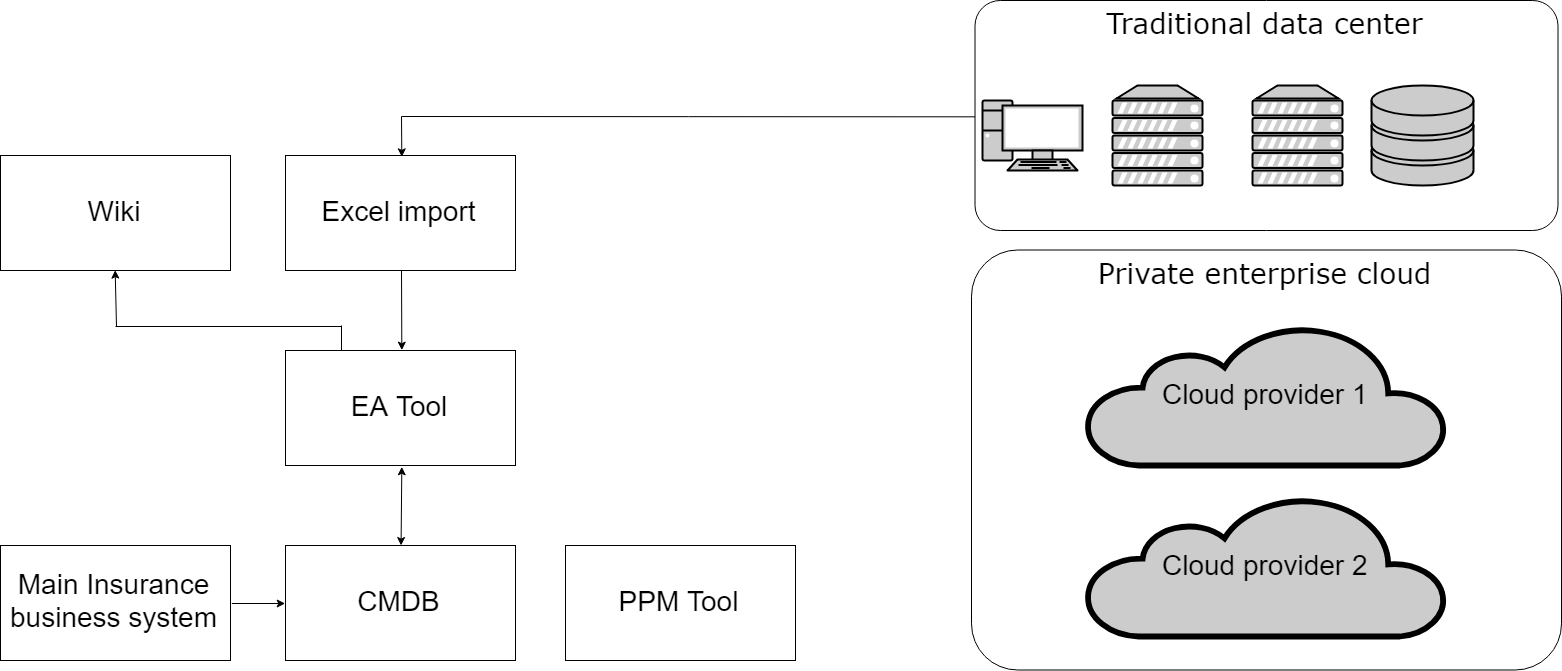
\includegraphics[width=1.0\textwidth]{figures/as-is-it-landscape.png}
  \caption{ AS-IS IT landscape}
  \label{fig:AS-IS IT landscape}
\end{figure}

The company consists of two environments: the traditional environment which contains traditional data center hardware and its private cloud infrastructure which is divided into two different cloud service providers. The first cloud infrastructure service provider is Redhat's OpenShift\footnote{\url{https://www.openshift.com/}} and the second provider is Pivotal's CloudFoundry\footnote{\url{https://www.cloudfoundry.org/}}.

The traditional data centers host the legacy systems of the company and all other kind of applications.

OpenShift is a container platform. The PaaS provider OpenShift offers the possibility to deploy docker containers to its platform and enables the orchestration by Kubernetes\footnote{\url{https://kubernetes.io/}}.

CloudFoundry (CF) is an open source, multi-cloud application platform as a service. Similar to Openshift, CF has a container-based architecture which also enables the deployment of applications written in any programming language.

The main components of the IT landscape shown in figure~\ref{fig:AS-IS IT landscape} in regard to EAD are the EA tool, the CMDB, the PPM tool, 
%a service-oriented architecture (SOA) repository, 
the Wiki s a collaboration software program and the main business system. 

\subsection{Current EA documentation}\label{subsection:currentead}

The EAD integrates several tools as shown in figure~\ref{fig:AS-IS IT landscape}. 

\subsubsection{Excel import}

The first EA documentation process was driven by the external mentioned ISO 22301 standard. The enterprise decided to collect the information about the IT landscape. The usage of Microsoft Excel sheets for keeping data is still important for enterprises since many organizations still rely on them for information storing. \cite{Farwick2013}

Initially the systems or applications that are critical for the business were documented. This was mainly driven by the BCM project and the BIA of IT failures. Ensuring that important business process are not interrupted and have no economic impact to the company is essential that the enterprise remains secure. Due initiative a team was created to retrieve this information. The documentation process was done fully manually. Therefore the document containing the information was inconsistent and contained redundant information.

The continuation of the project is mainly driven by the VAIT regulation since enterprise will have to have a complete application inventory.

\subsubsection{Integration of the CMDB}
% Pasarlo a current EA docu?
Due to the BCM regulation mentioned in section~\ref{subsection:internalinfluencingfactors}, an integration between the EA tool and the CMDB was implemented. The EA tool integrates data from the CMDB. The application developed for the integration retrieves data from the CMDB and imports the data to the EA tool in regular intervals. The import was unidirectional. Only Business Services were imported from the CMDB. A Business Service is a metamodel object in the CMDB. No infrastructure data was integrated into the EA tool. The import did not analyze the data, meaning that if the imported data was redundant there was no merge conflict solved. The integration was further developed to improve these challenges. The Integration on the CMDB contains now a conflict solution and harmonizes the redundant imported applications with a unique identifier. The import mechanism also differentiates between a flag set in the CMDB metamodel to import the business services as an application or a technical components. This differentiation is done because in the CMDB everything was modeled as a business service.

This integration was the pilot integration project for information sources to the existing EA tool. Further integrations of different information sources will be implemented due to the successful development of this integration.

The main business system of the enterpise was initially documented in the CMDB. For that reason the information about the main business system was retrieved via the CMDB to the EA tool.

%Semi automated?
The integration of the CMDB to the EA tool is seen as semi-automated since the information of the CMDB was retrieved manually.

\subsubsection{Export to Wiki}

The export of the collected data in the EA tool was mainly driven by the integration of the CMDB. The goal of the data export to the Wiki was to analyze and evaluate the data of the EA tool. 

Enterprise Wikis enhances sharing and collaboration of employees knowledge. The employees can easily edit the wikis content and provide their knowledge to the information center. The unstructured information can contain file attachments, multimedia content and allows the interlinkage of wiki pages. Referencing EA relevant information such as documents is supported by wikis. To link this references wikis are more appropriate than an EA tool. \cite{Fiedler2013}

To enable the collaboration and knowledge sharing of the employees knowledge a Wiki was integrated into the IT landscape. A wiki page is created for each application of the EA tool. This enables to collect more data than the metamodel of the EA tool allows. The wiki page contains several characteristics of an application. Some of the extended characteristics of an application are architectural decision, users, architectural diagrams, decommissioning information driven by the decommission concern, operational manual and other notes regarding the application.

\subsubsection{Cloud integration}

As illustrated in figure~\ref{fig:AS-IS IT landscape} there is no integration of the applications running on the cloud-based environments. There is no defined process of the EAD of applications deployed to the cloud.

In the context of the cloud migration project a new defined process for the deployment of the new developed applications was introduced. The major goal of this defined process is to establish a standardized process for agile teams. The process is divided into a build process and a deployment process.

\begin{figure}[htpb]
  \centering
  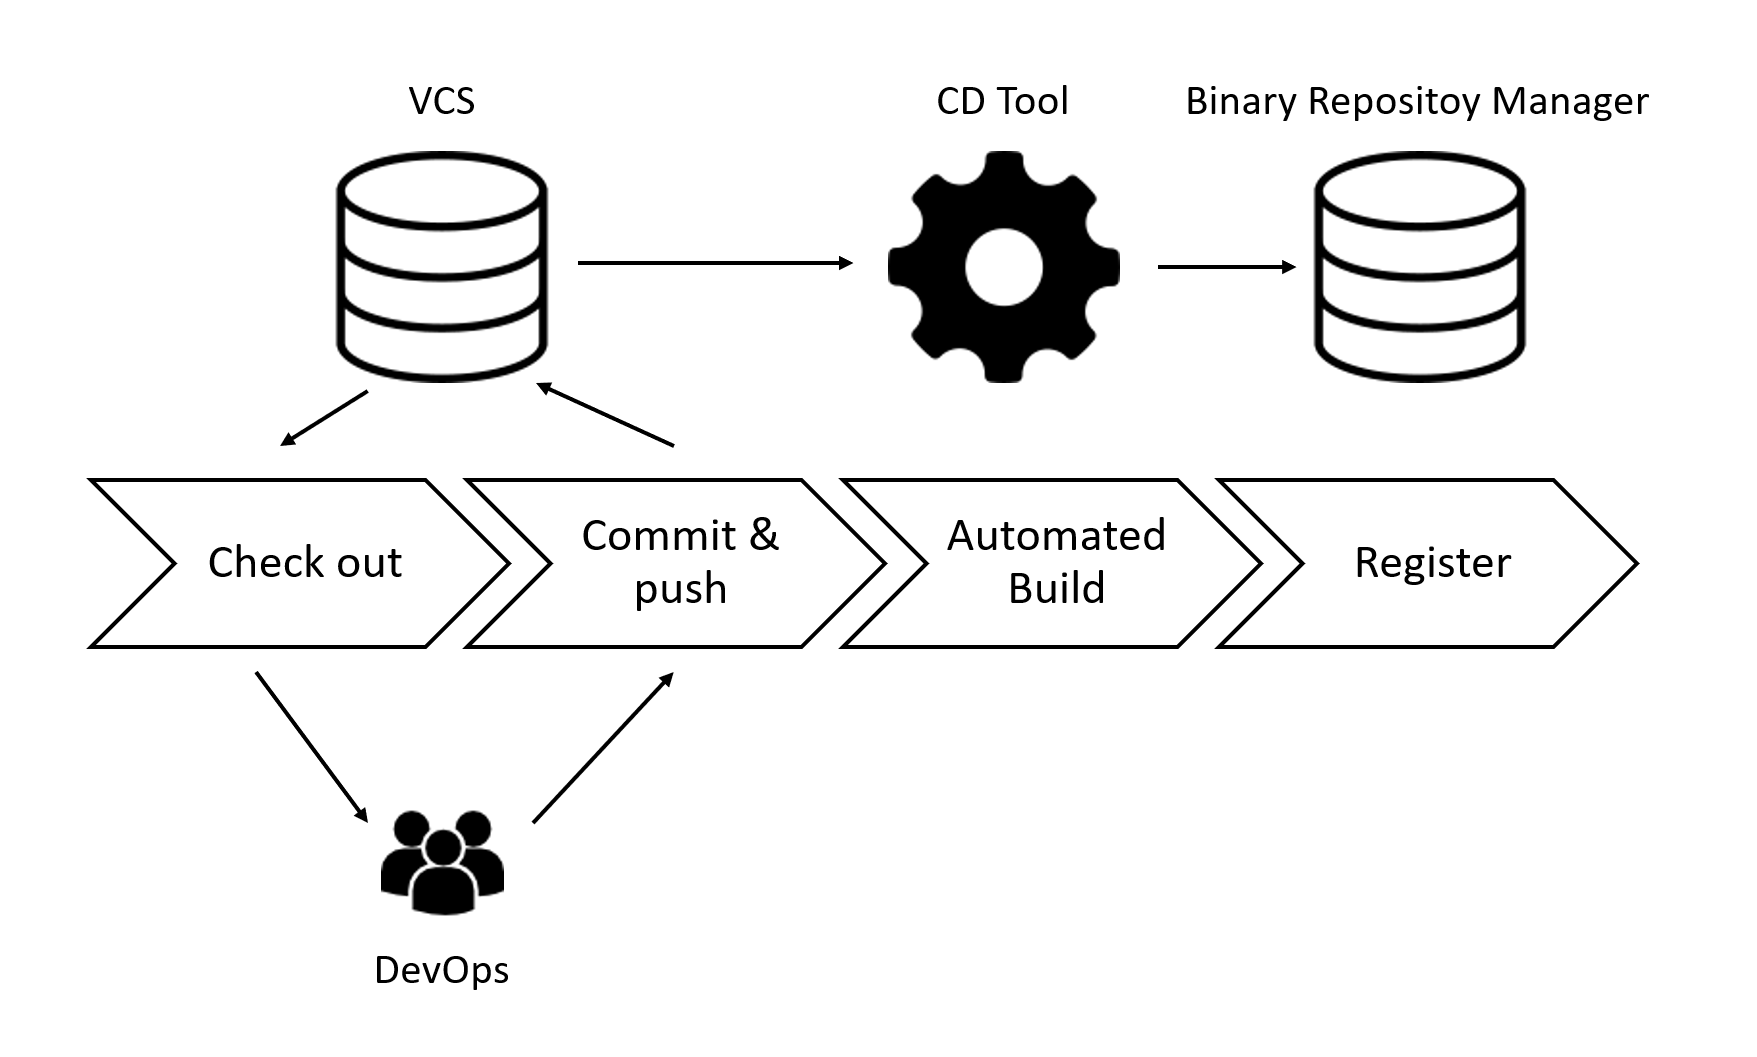
\includegraphics[width=0.8\textwidth]{figures/build-process.PNG}
  \caption{ Build process}
  \label{fig:Build-process}
\end{figure}

The build process is shown in figure~\ref{fig:Build-process}. The DevOps team first checks out the latest state of the code from the version control service (VCS). After developing the team commits and pushes the new state back to the VCS repository. The CD tool is constantly monitoring the repository to track changes in the code. If new changes are tracked, the CD tool automatically builds an artifact of the repository and registers the artifact into the binary repository manager tool. That means the built artifact is hosted in the tools and can be downloaded from it.

\begin{figure}[htpb]
  \centering
  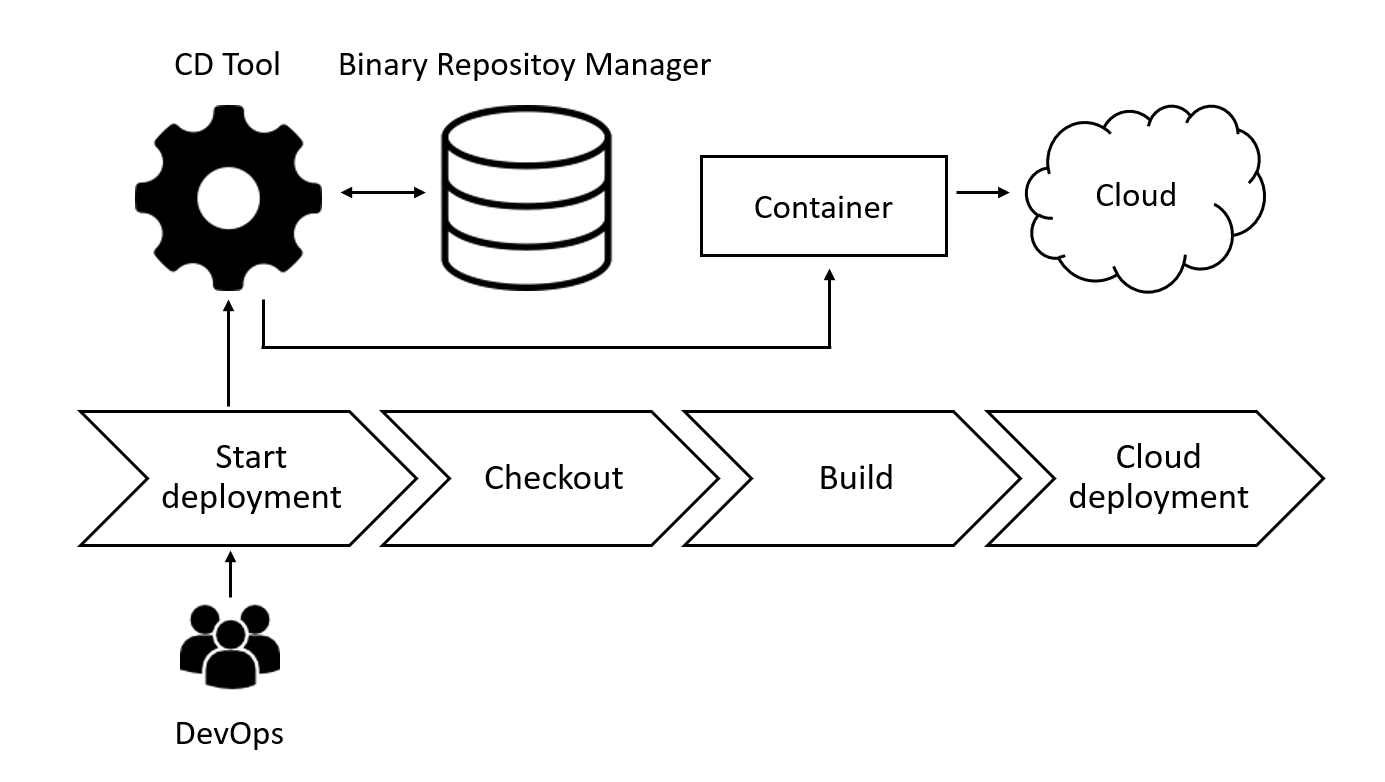
\includegraphics[width=0.8\textwidth]{figures/deployment-process.PNG}
  \caption{ Deployment process}
  \label{fig:Deployment-process}
\end{figure}

The second part of the defined process is the deployment process as shown in figure~\ref{fig:Deployment-process}. The DevOps team triggers manually the deployment process within the CD tool. The tool downloads the latest pushed artifact of the binary repository manager. After downloading the artifact, it build automatically a container out of the artifact. The CD tool pushed then the container to the cloud.

The first approach for a documentation process of the applications running on a cloud-based environment is the establishment of a defined process and a toolchain for building and deploying to the cloud infrastructure. Every application is tracked in the binary repository manager but there is still no integration of the cloud application inventory to the EA tool.

\subsubsection{PPM Tool integration}

As figure~\ref{fig:AS-IS IT landscape} shows, there is no integration of a PPM Tool. Projects and business information can not be aligned to applications during the EAD.

\section{Target IT landscape}\label{section:targetitlandscape}

This section will explain the target IT landscape of the company. The target IT landscape is mainly driven by the concerns. The following picture shows the target IT landscape in regard to EAD.

\begin{figure}[htpb]
  \centering
  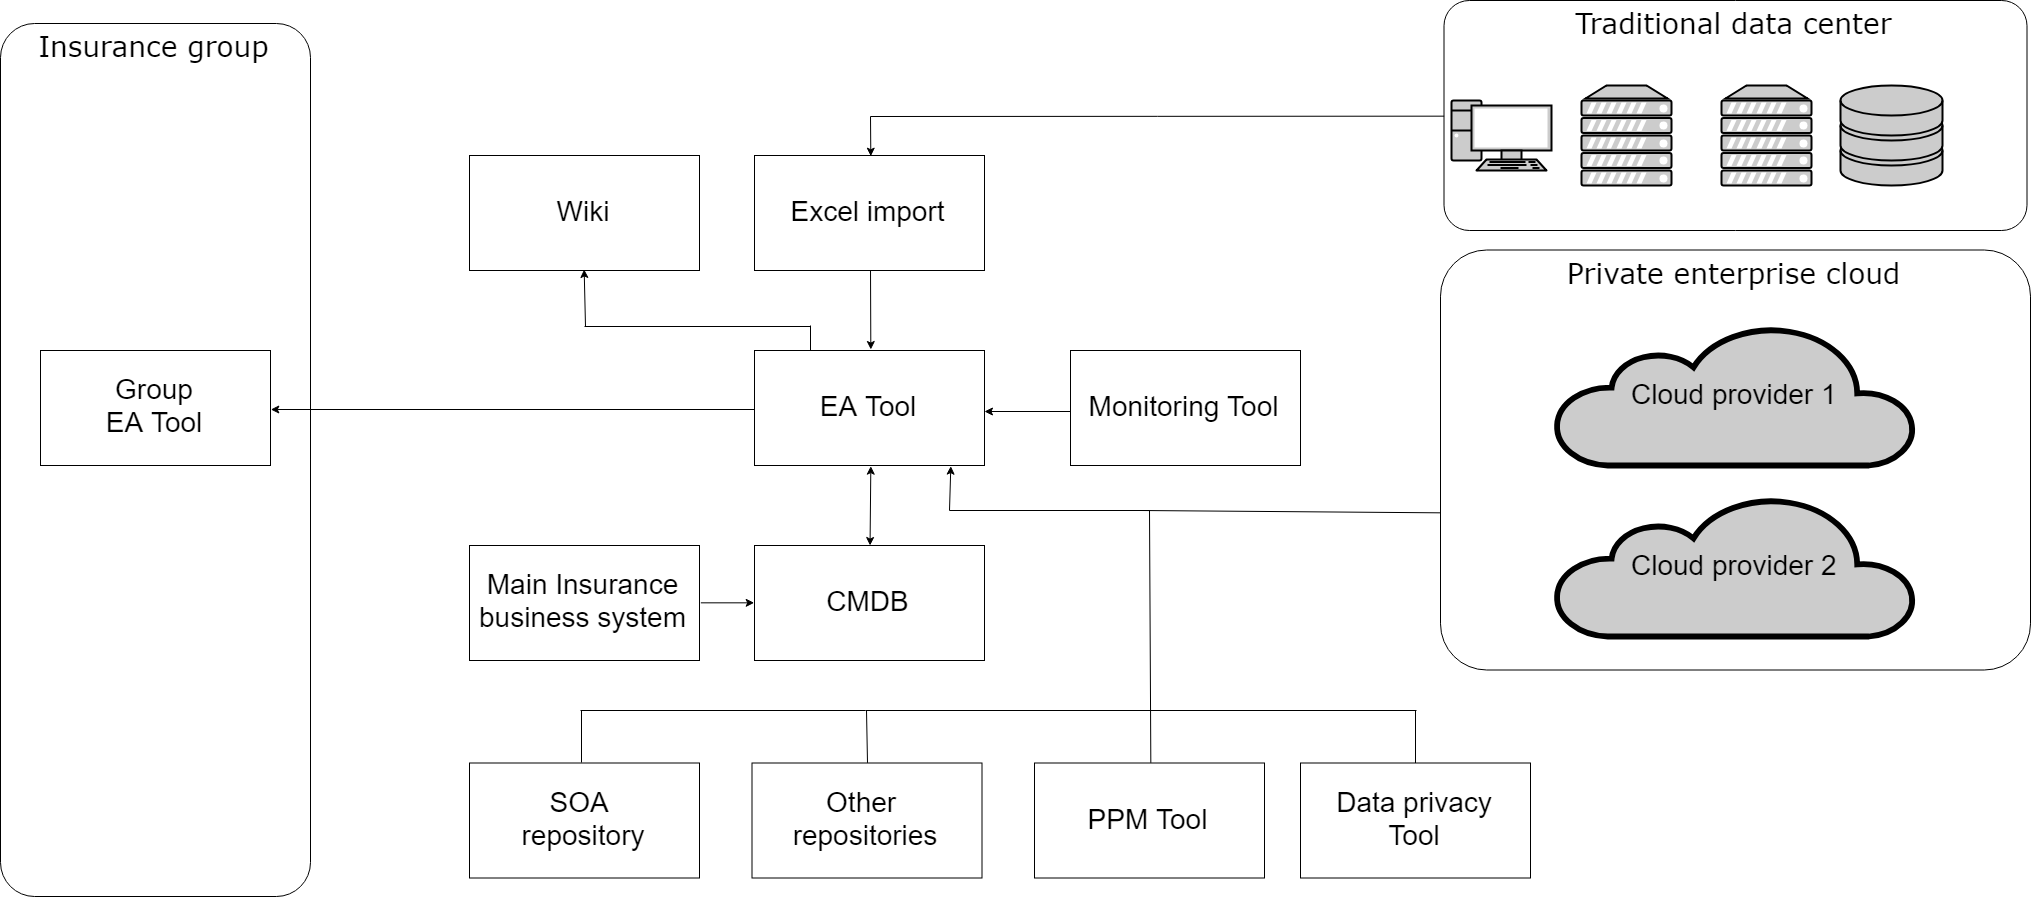
\includegraphics[width=1.0\textwidth]{figures/target-it-landscape.png}
  \caption{ Target IT landscape}
  \label{fig:Target IT landscape}
\end{figure}

\subsubsection{Integration of data privacy tool}
%Amur für datenschutz
Driven by the GDPR the enterprise has developed a tool which contains a list of applications that are related to this regulation. Therefore an integration of this tool is planned in order to have this specific information in the EA tool.

\subsubsection{Integration of service-oriented architecture repositories}

An integration of a service-oriented architecture (SOA) repository is intended.
The SOA repository is used for managing services such as WSDLs and XML schema definitions, access rights, information related to the service level agreements and transactional operations of the services. \cite{Krafzig2005} 
%Enterprise SOA: Service-oriented Architecture Best Practices By Dirk Krafzig, Karl Banke, Dirk Slama

\subsubsection{Integration of other repositories}
The enterprise goal of the enterprise is to interlink different tools containing different EA relevant information. This goal enables a federated architecture to allow information sharing between different data sources. Therefore it will also integrate other repositories such as license management tools and change management tools.
%Relevant for the EAD are also the other repositories depicted in the figure~\ref{fig:AS-IS IT landscape}. Other repositories include change management tools, license management tools, etc.

\subsubsection{Integration of the PPM tool}
The main goal of the integration of a PPM Tool is to enable a mapping between the projects and the applications or systems in the enterprise. The EA tool in place contains in its metamodel the entity "project". This allows an integration of the PPM tool to the existing EA tool. The projects of the PPM tool are imported into the EA tools as the entity "project". A manual mapping between the projects and applications is then still required. This EAD process of projects can be seen as semi-automated.

\subsubsection{Integration to the group EA tool}

The insurance company is divided into several subsidiaries around the world. The VAIT regulation is applied to every german insurance company. The company group is based Germany so the regulation implies an IT inventory for every subsidiary of the group. Therefore every operating entity (subsidiary) has to export the EA information to the Group entity.

\subsubsection{Cloud integration}

As shown in figure~\ref{fig:Target IT landscape} the applications running on the cloud-based environments will be integrated to the EA tool. The main driver for this integration is the VAIT regulation. As mentioned in the regulation, an insurance company has to be able to deliver an application inventory of the IT landscape. That includes also applications running on private enterprise clouds. 

\subsubsection{Monitoring tool integration}

The introduction of a monitoring tool is planned. The reason for establishing a monitoring tool is to gain advantage over the competitors. Monitoring applications allow to retrieve extra information such as individual requests and transactions, resource consumption, reporting and alerting, etc.

The business benefits of monitoring tools for the enterprise are many. One of the benefits is that the enterprise can react quicker to an application failure reducing the revenue loss due to the breakdown of the respective applications or systems. Knowing the failures and obtaining the dependencies from the monitoring tool the enterprise can derive what other systems will be affected by the breakdown. This matches the requirements from the BCM project.

\section{Derived requirements}\label{section:derivedrequirements}

In the previous sections the as-is and target landscape of an insurance company were presented. These sections cover various aspects of the EAD within the studied company. The case study shows different outlooks for future integrations. From the introduced case study, requirements can be derived for an automated EAD. The following table presents the derived requirements:

\begin{table}[htpb]
  \caption[Automated EAD requirements derived from the case study]{Automated EAD requirements derived the case study}\label{tab:casestudyrequirements}
  \centering
  \begin{tabular}{l l l}
    \toprule
      Id & Requirement\\
    \midrule
      %RC1 & Business Impact Analysis of applications\\
      %RC2 & Data privacy compliance\\
      RC1 & Integration of a PPM tool\\
      RC2 & Integration of different information sources\\
      RC3 & Integration of cloud infrastructure\\
      RC4 & Integration of a monitoring tool\\
    \bottomrule
  \end{tabular}
\end{table}

\textbf{RC1}: The integration of a PPM tool is desired by the enterprise to relate projects to applications.

\textbf{RC2}: An integration of different information sources is required by the enterprise to relate information and propagate information sharing.

\textbf{RC3}: The integration of cloud infrastructure is needed due to a full application inventory required by law and due to strategic decisions as migrating to cloud infrastructure.

\textbf{RC4}: An integration of a monitoring tool is planned at the enterprise to increase the reaction time between the failure of a system and the enterprise. Thus, the monetary impact can reduced.

The requirements from the insurance company  can be aligned to the requirements derived during the literature research. \textbf{RC1} and \textbf{RC2} can be mapped to \textbf{RL1} since the requirements propose the integration of different information sources. \textbf{RC1} is just a special requirement of the integration of various data sources. \textbf{RC3} and \textbf{RL5} can be aligned since both requirements demand an integration of cloud environments. \textbf{RC4} and \textbf{RL6} require an enhancement of runtime KPIs through monitoring tools.
In summary, the enterprise requirements can be aligned to the findings of the literature research and the respective derived requirements. 

\section{Case study evaluation}\label{section:solutionarchitecture}

This section will evaluate the implemented prototype of chapter~\ref{chapter:prototype implementation} within the studied enterprise. The first subsection will introduce the methodology and the overall goal of the evaluation. The second subsection will present the results of the prototype evaluation.

\subsection{Evaluation goal and methodology}


The goal is to evaluate the presented approach and the implemented prototype in the case to see whether the approach and the prototype are a valuable solution for improving the automation of EAD. To test the prototype stakeholder were interviewed. The interview was structured in three parts. The first part was an introduction of the approach. The second part of the interview was a presentation of the tool. The third part was the actual interview of the stakeholder based on a evaluation questionnaire of the developed solution. The evaluation questionnaire is attached in Appendix~\ref{section:evaluationquestionnaire}. 

Nine enterprise architects and three product owners were interviewed to obtain beneficial feedback. Table~\ref{tab:interviewedindustrypartners} shows the interviewed industry partners, their roles, the years of experience (YoE) as enterprise architects or product owners and the enterprises (E) they work for. The table shows that the maturity of most of the interviewed enterprise architects is high. Different to the enterprise architects, most of the product owners were not that experienced but could deliver some innovative ideas.
All of the interviewed industry partners work in insurance companies.

\begin{table}[htpb]
  \caption[Interviewed industry partners evaluation]{Interviewed industry partners evaluation}\label{tab:interviewedindustrypartners}
  \centering
  \begin{tabular}{l l l l l}
    \toprule
      No & Pseudonym & Role & YoE & E\\
    \midrule
      1 & EA1 & Enterprise Architect and Chief Architect & 20 & E1\\ %Hansrudi
      2 & EA2 & Enterprise Architect & 2 & E1\\ %Christina
      3 & EA3 & Enterprise Architect & 17 & E1\\ %Kai
      4 & EA4 & Enterprise Architect and Product Owner & 10 & E1\\ %Martin
      5 & EA5 & Enterprise Architect & 5 & E1\\ %Matheus
      6 & EA6 & Enterprise Architect and IT Management Expert & 20 & E2\\ %Monika
      7 & EA7 & Enterprise Architect & 18 & E1\\ %Wolfram
      8 & EA8 & Enterprise Architect & 16 & E3\\ %Bart
      9 & EA9 & Enterprise Architect & 30+ & E4\\ %John    
      10 & PO1 & Product Owner and Head of Product Architecture & 11 & E1\\ %Christoph
      11 & PO2 & Product Owner & 1 & E1\\ %Max
      12 & PO3 & Product Owner & 3 & E1\\ %Simon
    \bottomrule
  \end{tabular}
\end{table}

\subsection{Approach evaluation}

As mentioned before a part of the interviews was the presentation of the approach on how to automate the EAD. This subsection will give the overall results of the evaluation questionnaire regarding the approach.

%Effort for EAD
At the beginning of the interview some general questions regarding EAD were asked. When the experts were asked about the effort for documenting the IT landscape of their company, 10 experts strongly agreed and 2 of them agreed. This means that the effort to document the landscape is still seen as an exhausting task. 
%Information outdated

A similar answer was given when the experts were asked about the actuality of the EA information. 10 of 12 experts answered that the EA information is outdated and 2 of them replied that it is partially outdated.

%-----------------------------------------------------------
%CD approach
%cloud usage
%migration of legacy systems to cloud 
%--------------------------------------------------------------
All of the interviewed experts replied that their company follow a CD approach (questions 2.1) and over 80 percent of the experts stated that their enterprises use cloud environments for deploying new developed applications or for the migration of legacy systems (question 1.6 and 1.7).

The answered of the experts during the case study and the interviews were validated during the case study.

%Automated process for EAD
% CMDB import - partially seen as automated process
In regard to automated EAD, the definition is not perceived the same way by the experts. 6 experts denied to have an automated process for documenting the EA while 6 agreed to the question if the company has an automated EAD. All experts know that the data from the CMDB is imported to the EA tool but the opinions on the import as an automated EAD disagree because the data in the CMDB was gathered manually. 

%who collects EA info: Tabelle
During the interview the experts were asked (question 2.2) to determine the responsible person for documenting new developed applications in the EA Tool. Table~\ref{tab:eadresposible} shows that the role of documenting the EA is not clearly defined.
\begin{table}[htpb]
  \caption[Question: Who collects the EA information of a new developed application/service for the EA Tool?]{Question: Who collects the EA information of a new developed application/service for the EA Tool?}\label{tab:eadresposible}
  \centering
  \begin{tabular}{l l l l l}
    \toprule
      Pseudonym & EA & PO & DevOps & Other\\
    \midrule
      EA1 &  & & X &\\ %Hansrudi
      EA2 & X & & &\\ %Christina
      EA3 & & X & & Application owner\\ %Kai
      EA4 & X & X & X & Application owner\\ %Martin
      EA5 &  & & & Application owner\\ %Matheus
      EA6 & X & X & & Application owner\\ %Monika
      EA7 & & & X & \\ %Wolfram
      EA8 & X & & & \\%John 
      EA9 & X & & & Application owner\\%Bart 
      PO1 & X & & &\\ %Christoph
      PO2 & X & & &\\ %Max
      PO3 & X & & &\\ %Simon
    \bottomrule
  \end{tabular}
\end{table}

More than half of the enterprise architects responded that the "application owner" should document the new developed applications.
As a result of that, the interviewed experts were inquired (question 2.10) to was explain how the application owner is determined. The application owner is the responsible person from the business side. This answer supports the business and IT alignment of the EA documentation since the experts struggle to determine the adequate person of the business part.

One of the experts replied to this questions that either you find the right information in the wiki or by "knowing the organization very well." This answer sums up and reinforces again the need for a business alignment.

\subsubsection{Information sources}

The experts were also interviewed about the information sources they use and would like to use and/or integrate.
In question 2.3 the experts were asked if they use any of the mentioned information sources to retrieve EA relevant information.
Figure~\ref{fig:question23} shows the answers of the experts regarding the usage of the EA relevant information sources according to the information sources mentioned by literature. \cite{Farwick2013}

The reason why the CMDB reached a high number of answers is because most of the interviewed industry partners belong to the german insurance company used for the evaluation which is depicted in the table as \textbf{E1}. The same reason explains the null value of the ESB. E1 has no established ESB in the enterprise. According to the results the other enterprises (E2, E3, E4) do not have an ESB in place. However, an ESB is considered as a n EA relevant information source. \cite{Hauder2013}
Most of the experts use a PPM tool as a EA relevant information source but document the information manually in the EA tool.

\begin{figure}[htpb]
\centering
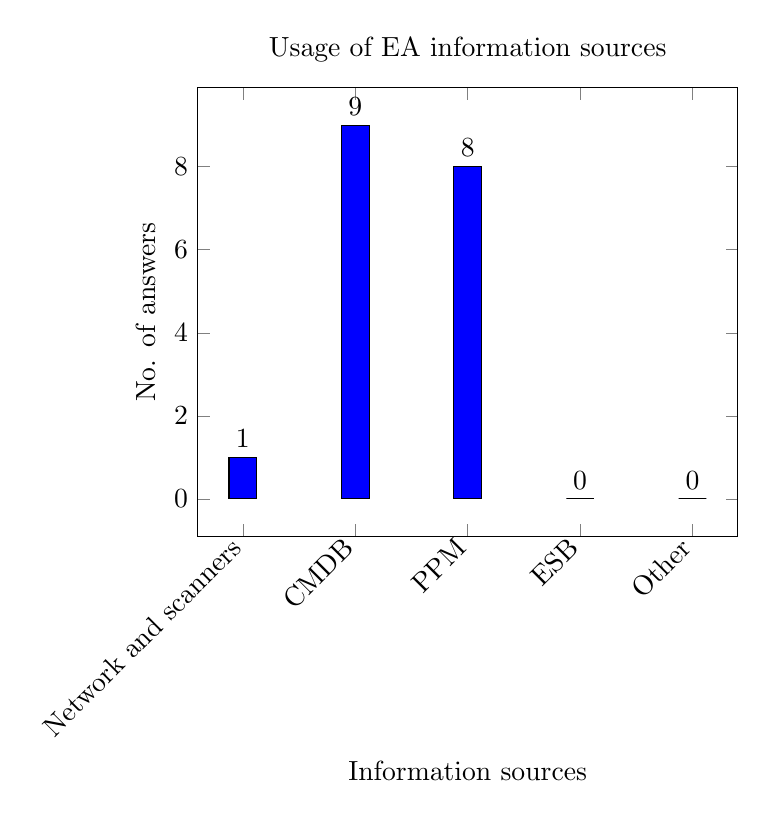
\begin{tikzpicture}
\begin{axis}
[
    title={Usage of EA information sources},
    xtick=data,
    symbolic x coords={Network and scanners, CMDB, PPM, ESB, Other},
	ylabel=No. of answers,
	xlabel=Information sources,
	x tick label style={rotate=45,anchor=east, align=center},
	nodes near coords,
	nodes near coords align={vertical},
]
\addplot 
    [ybar,fill=blue]
	coordinates {(Network and scanners,1) (CMDB,9)
		 (PPM,8) (ESB,0) (Other,0)};
\end{axis}
\end{tikzpicture}
\caption{Question 2.3: Do you use any of the mentioned information sources to retrieve EA relevant information?}
\label{fig:question23}
\end{figure}


%2.4 tools 2: 9 yes, 1 no but would like to use it. 
% 5 Wiki, 4 Jira, 3 Github, 2 Runtime -> Bar Chart
% manually 2, 1 expects the EA to do the docu
In addition to question 2.3 the experts were also asked if the information sources shown in figure~\ref{fig:question24} also contain EA relevant data. Over 80 percent of the experts agreed. Figure~\ref{fig:question24} shows how often these additional information were named.

\begin{figure}[htpb]
\centering
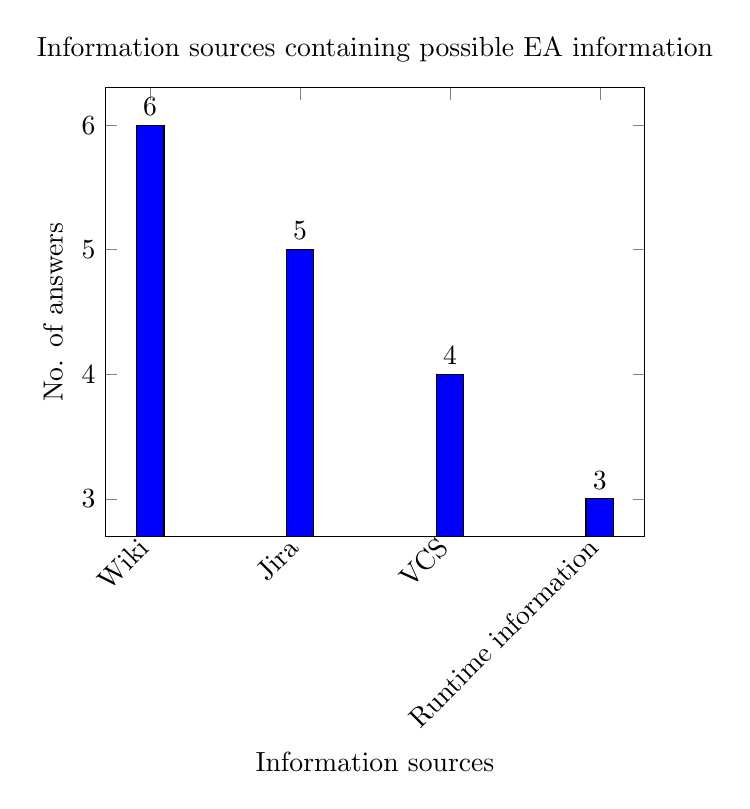
\begin{tikzpicture}
\begin{axis}
[
    title={Information sources containing possible EA information},
    xtick=data,
    symbolic x coords={Wiki, Jira, VCS, Runtime information},
	ylabel=No. of answers,
	xlabel=Information sources,
	x tick label style={rotate=45,anchor=east},
	nodes near coords,
	nodes near coords align={vertical},
]
\addplot 
    [ybar,fill=blue]
	coordinates {(Wiki,6) (Jira,5)
		 (VCS,4) (Runtime information,3)};
\end{axis}
\end{tikzpicture}
\caption{Question 2.4: Do you think this information sources could contain relevant EA information?}
\label{fig:question24}
\end{figure}
%2.5 How do you collect the information: 2 manually, 8 kA
Moreover, only 3 of the experts integrate the EA relevant information of the tools into the EA tool manually (question 2.5). The rest of the experts did not give an answer to that question and only PO3 expects that the enterprise architects should document the EA relevant information of the information sources mentioned in figure~\ref{fig:question24}.

% established toolchain: 10 yes, 2 no.
\subsubsection{Application development pipeline}
The experts were asked if their company had an established toolchain. More than 80 percent of the interviewed industry partners confirmed it. Figure~\ref{fig:comparison-approaches} shows the approach of this work in comparison to the pipeline of the case study of section~\ref{section:casestudy}.

%COMPARE approaches:
There are some differences regarding both approaches. The first difference is that in the pipeline of the case study the build process is triggered automatically after new changes were committed to the repository. The build process of the presented approach is triggered manually because not every change in the repository needs to generate a new artifact. After the build process is triggered in the pipeline of the presented approach the business information of the PPM tool is retrieved. This supports the statements of the interviewed experts to aggregate the information of PPM tool to an artifact. Another difference is that in the pipeline of the presented case study the built artifact is registered and stored in a Binary Repository Manager (BRM). Before starting the deployment process a container is built to wrap the application. The container is then deployed to the cloud. In the presented approach no container is built to wrap the application and the deployment process is automatically triggered. After the deployment the runtime information is gathered and it is aggregated to the other information collected throughout the pipeline. The aggregation of that information is then pushed to the tool used for an automated EAD.

\begin{figure}[htpb]
  \centering
  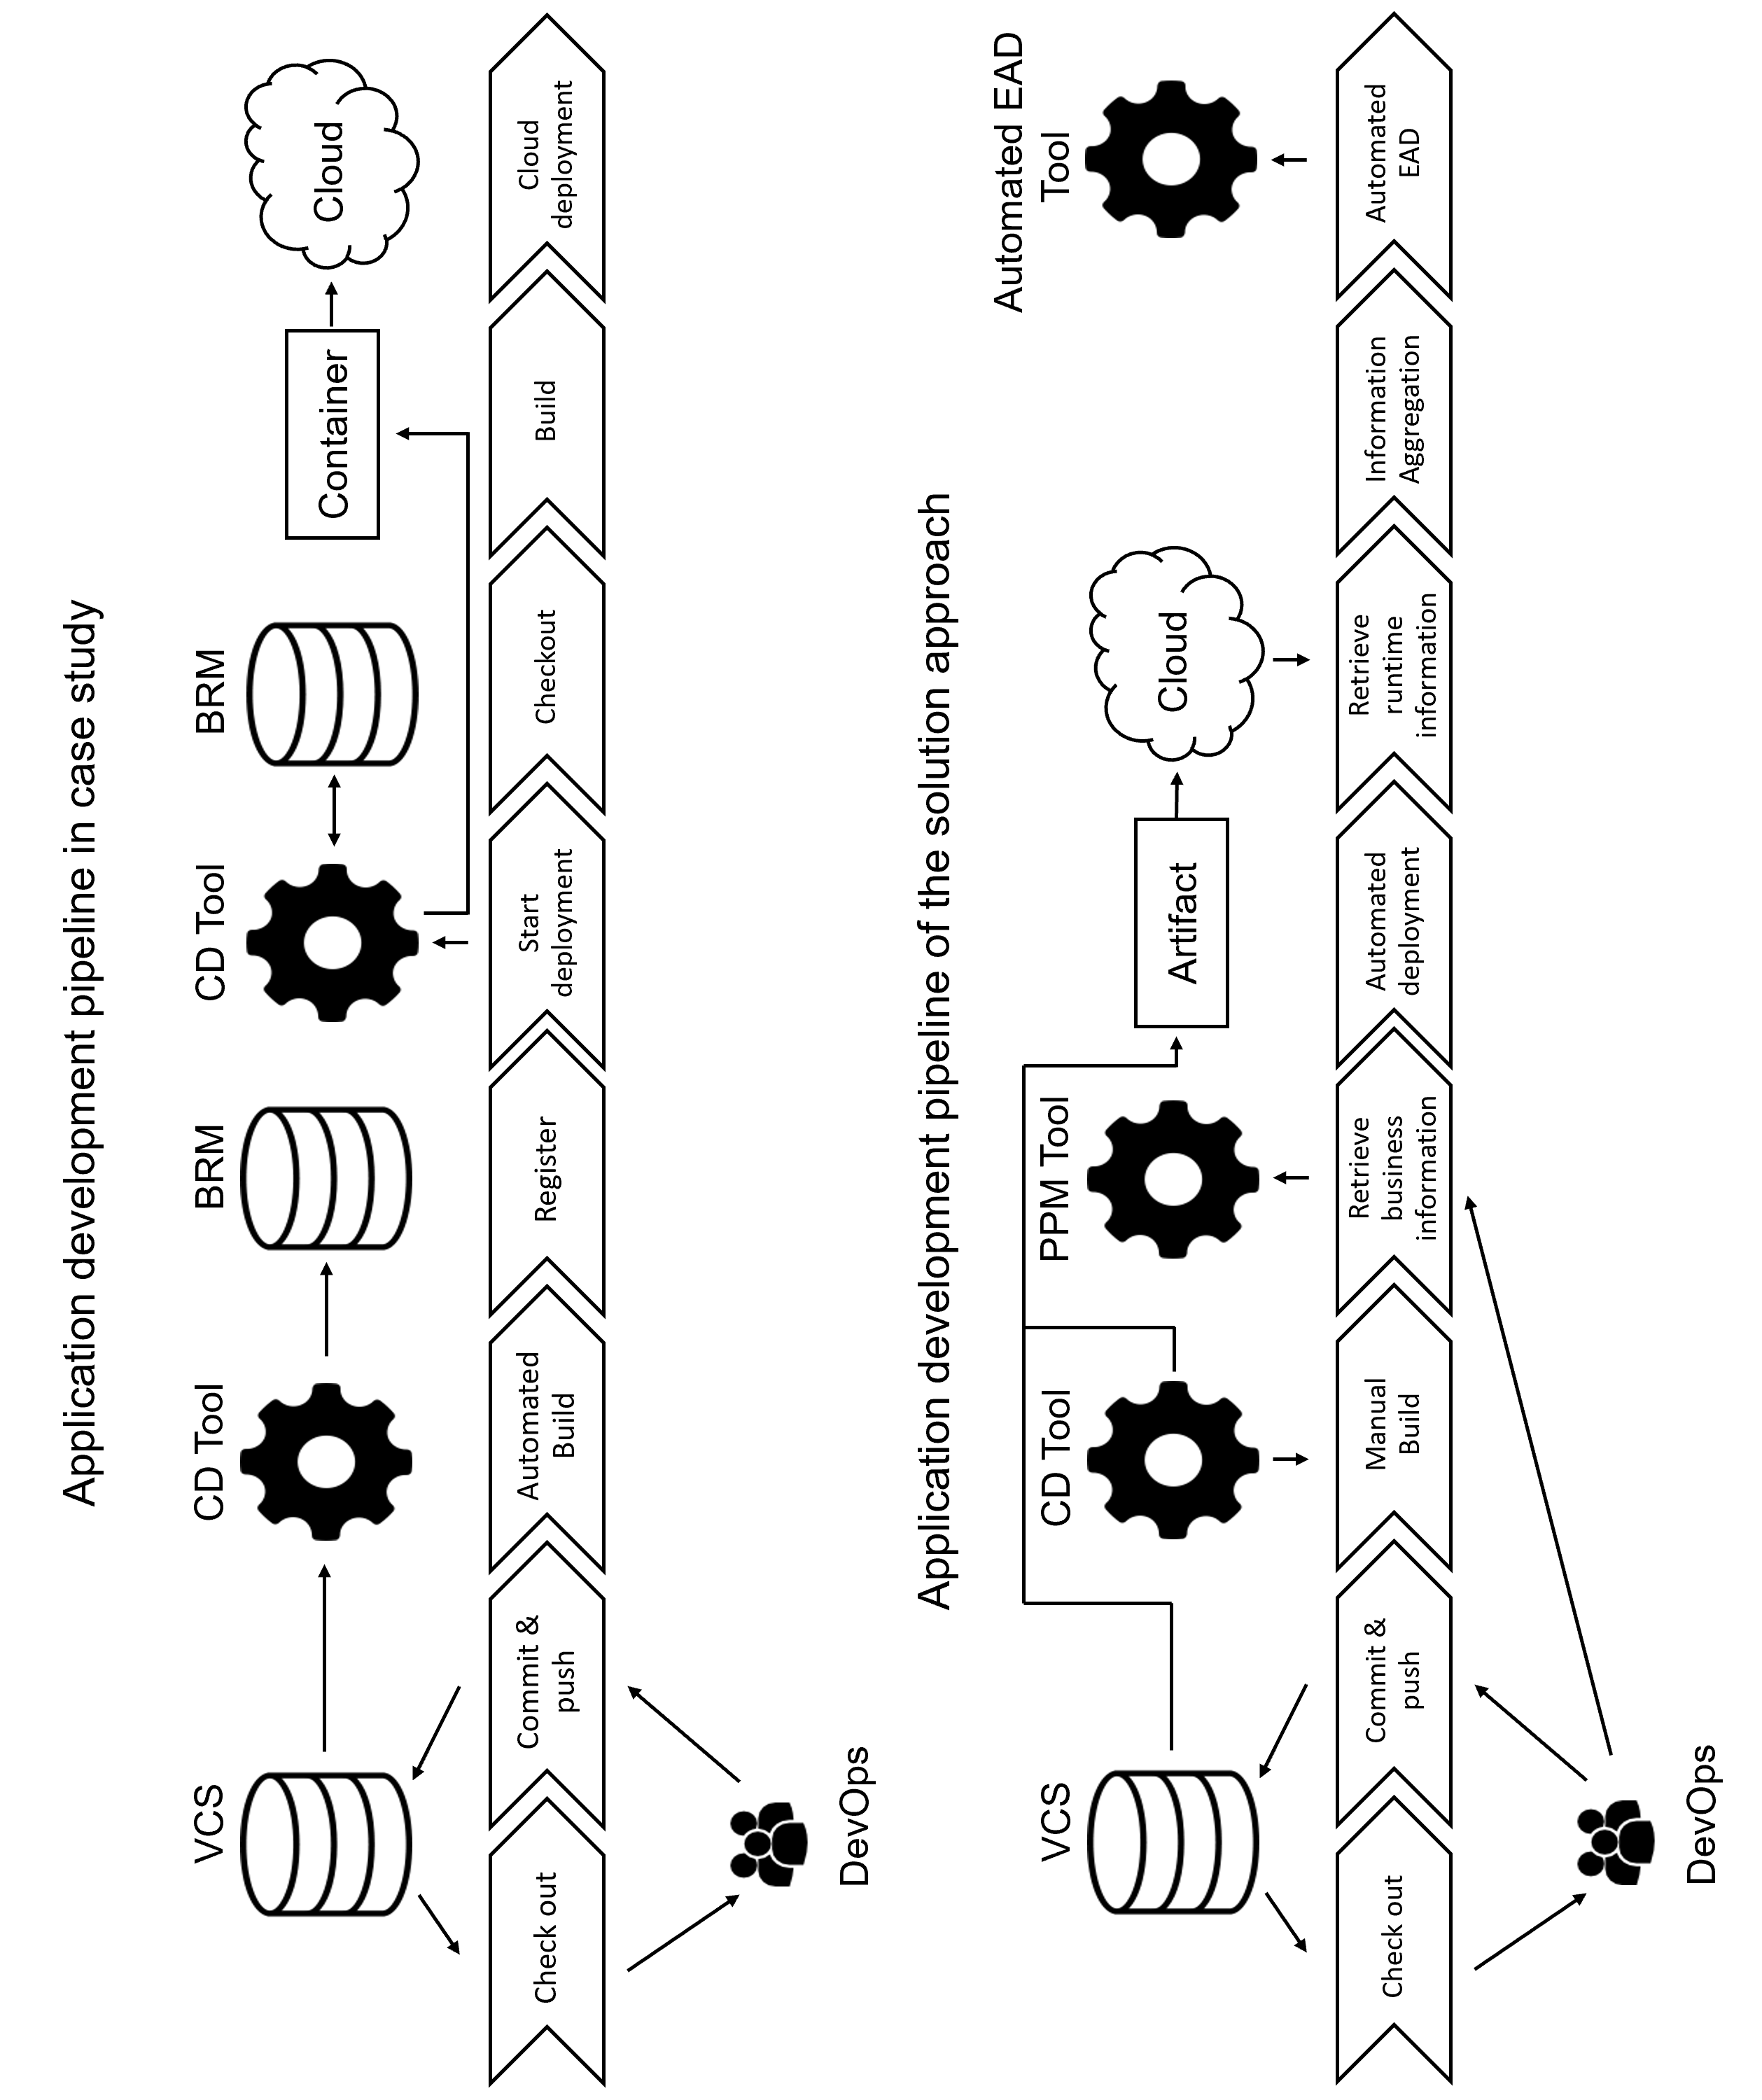
\includegraphics[width=1.0\textwidth]{figures/evaluation/comparissonapproaches.png}
  \caption{ Comparison of approaches}
  \label{fig:comparison-approaches}
\end{figure}

% established toolchain would improve this: 12 yes!
All of the industry partners confirmed that an established toolchain improves the process of EA documentation (question 2.7). The most frequently named reasons why it improves the EAD are standardization and automation (question 2.7). An established toolchain automates the EAD by introducing a standardized process. This reduces the manual effort mentioned in literature. \cite{Hauder2012} In also increases the data quality (DC4) and the data actuality (DC2). 
%Why?
%Automation and quality gates, Standardization and automation
%EA information which is documented automatically is more up-to-date. Increase of data actuality.
%Automation would help to standardize the process of documentation too. No extra effort needed.
%Starting from technical descriptions and application information data you can support building different views for different purposes.
%Standardization makes EA easier, it’s a central place to add policies across teams.
%Abzug von möglichst vielen bereits verfügbaren Daten wäre möglich

Further to question 2.6 the industry partners demanded to confirm the application of the approach mentioned in chapter~\ref{chapter:approach}, specially the imposition of the script for a predefined pipeline and the predefinition of the toolchain. Figure~\ref{fig:question28} shows the reactions to the statement if imposing the team to incorporate a pipeline-script in the repository is easy to establish.

\begin{figure}[htpb]
\centering
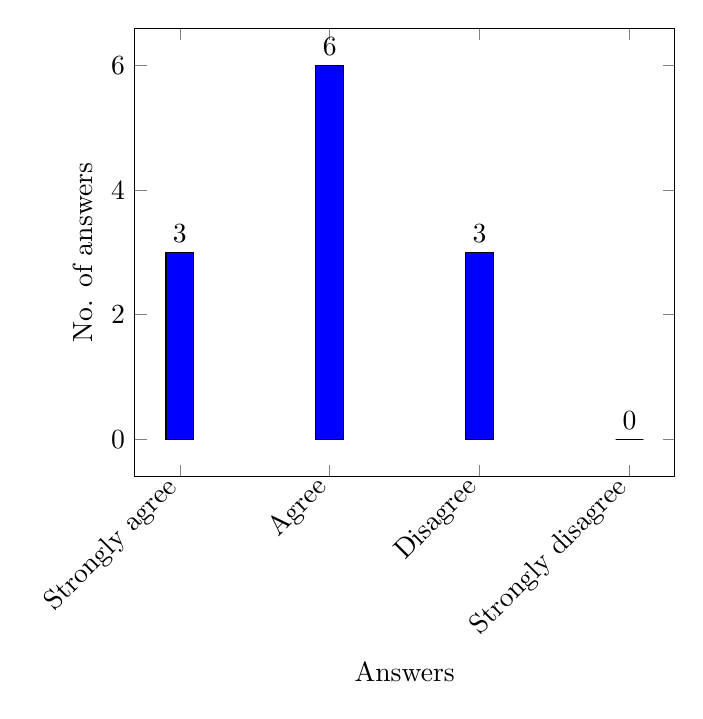
\begin{tikzpicture}
\begin{axis}
[
    %title={Imposing the team to incorporate a pipeline-script in the repository is easy to establish},
    xtick=data,
    symbolic x coords={Strongly agree, Agree, Disagree, Strongly disagree},
	ylabel=No. of answers,
	xlabel=Answers,
	x tick label style={rotate=45,anchor=east},
	nodes near coords,
	nodes near coords align={vertical},
]
\addplot 
    [ybar,fill=blue]
	coordinates {(Strongly agree,3) (Agree,6)
		 (Disagree,3) (Strongly disagree, 0)};
\end{axis}
\end{tikzpicture}
\caption{Question 2.8: Imposing the team to incorporate a pipeline-script in the repository is easy to establish}
\label{fig:question28}
\end{figure}


%predefined toolchain imposing: 6 agree, 2 Strongly agree, 2 disagree? -> Bar CHart. 2 disagree because difficult to establish in organization, not because of the team.
Figure~\ref{fig:question29} shows the answers in regard to the imposition of a predefined toolchain. The disagreed interviewed were asked about their disagreement and the disagreement concerns rather the establishment of a toolchain within a large enterprise, not about imposing the agile development teams to use a predefined toolchain.

\begin{figure}[htpb]
\centering
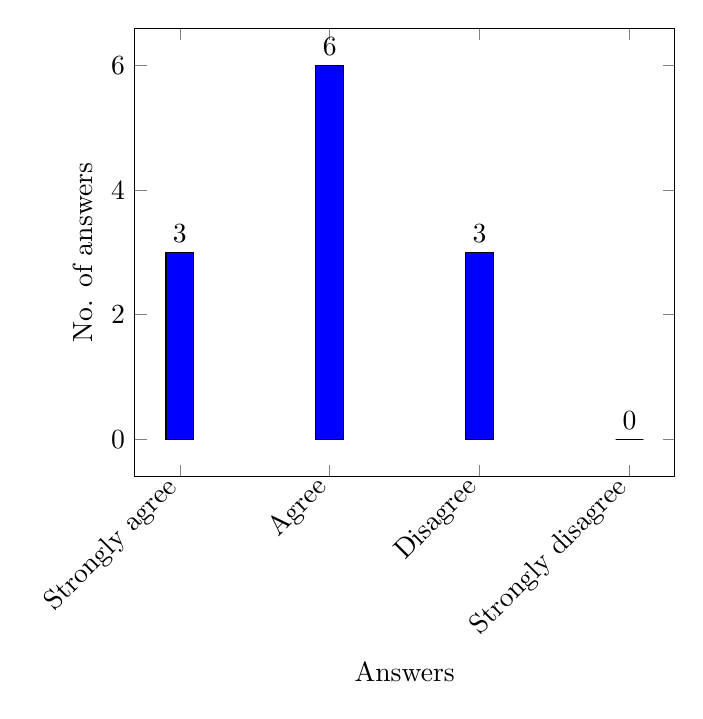
\begin{tikzpicture}
\begin{axis}
[
    %title={Imposing the team to use a predefined toolchain for the application development is easy to establish},
    xtick=data,
    symbolic x coords={Strongly agree, Agree, Disagree, Strongly disagree},
	ylabel=No. of answers,
	xlabel=Answers,
	x tick label style={rotate=45,anchor=east},
	nodes near coords,
	nodes near coords align={vertical},
]
\addplot 
    [ybar,fill=blue]
	coordinates {(Strongly agree,3) (Agree,6)
		 (Disagree,3) (Strongly disagree, 0)};
\end{axis}
\end{tikzpicture}
\caption{Question 2.9: Imposing the team to use a predefined toolchain for the application development is easy to establish}
\label{fig:question29}
\end{figure}

%4.2 enables federated approach: 6 agree 6 Strongly agree
\subsubsection{Federated EA}
Regarding a federated enterprise architecture all experts confirmed that the approach of this work enables it. 50 percent of the industry partners agreed to it and 50 percent strongly agreed.

%3.5 Do you use any technologies for monitoring applications?
%3.1 EAD of cloud apps: 3 manually, 7 garnicht.
\subsubsection{Cloud EAD}
8 of the interviewed industry partners use technologies for monitoring applications and the rest do not use technologies for monitoring applications or do not know about the usage of these technologies (question 3.5). 

During the interviews the experts were asked to list the monitoring technologies. The following "monitoring technologies" were listed:
\begin{itemize}
    \item Grafana\footnote{\url{https://grafana.com/}}
    \item Tivoli\footnote{\url{https://www.ibm.com/support/knowledgecenter/en/SSTFXA_6.3.0/com.ibm.itm.doc_6.3/welcome_63.htm}}
    \item Prometheus\footnote{\url{https://prometheus.io/}}
    \item ELK stack\footnote{\url{https://www.elastic.co}}
    \item Dynatrace\footnote{\url{https://www.dynatrace.com/}}
\end{itemize}

Grafana was the most mentioned technology. This shows that the experts do not know the definition of monitoring technologies. 
Grafana is a platform that allows the user to visualize, alert on and understand the applications metrics. Grafana does not monitoring the application itself.
The ELK Stack is consists three open-source products: Elasticsearch, Logstash, and Kibana. Elasticsearch is a NoSQL database, Logstash is a log pipeline tool and Kibana is a visualizes the Elasticsearch data. None of the mentioned products monitors the applications.
However, the other listed technologies do monitor applications.
Tivoli is a set of products from IBM that monitors the performance and availability of operating systems and applications.
Dynatrace monitors real user data, application performance, infrastructure and cloud environments.
Prometheus is an systems monitoring and alerting toolkit.

When it comes to the EAD of cloud applications 4 out of 8 industry partners using technologies for monitoring applications still document cloud applications manually.

%5.1 process automates EAD for clouds
All of the interviewed experts confirmed that the presented process automates the EA documentation of applications/services running on a cloud-based environment (question 5.1). 3 experts strongly agreed to the statement and 9 agreed.


\subsection{Tool evaluation}

This subsection will give an overview of the results of the evaluation regarding the implemented prototype. The same experts of table~\ref{tab:interviewedindustrypartners} were consulted about the implemented prototype for further development and improvement.

\subsubsection{Solution architecture of prototype}
Figure~\ref{fig:solution-architecture-prototype} shows the solution architecture of the prototype in the current IT environment of the insurance company.

\begin{figure}[htpb]
  \centering
  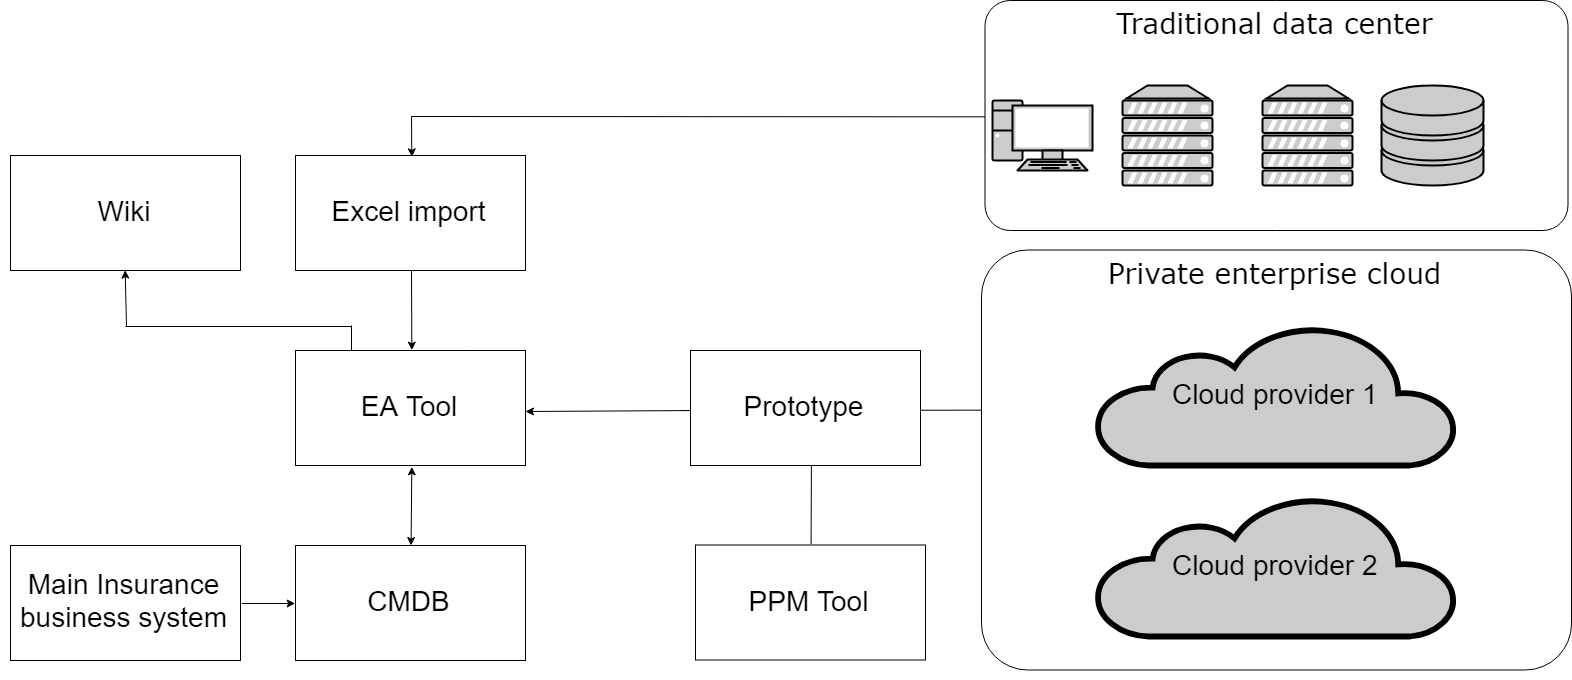
\includegraphics[width=1.0\textwidth]{figures/solution_architecture-prototype.png}
  \caption{Solution architecture of the prototype in the current IT landscape of the enterprise}
  \label{fig:solution-architecture-prototype}
\end{figure}

\subsubsection{Challenges of the prototype}\label{subsubsection:challenges-prototype}
The challenges of the prototype include governance aspects and implementation issues.

The first problem during the establishment of the tool was that the cloud were the prototype was deployed, did not allow to deployment and set-up of a MongoDB instance. Due to this reason a MySQL\footnote{\url{https://www.mysql.com/}} database component was used in the case study. The consequences of this was the adaptation the server component. 
The web component also needed some adjustments. The web-browser allowed at the company did not ECMAScript 6\footnote{\url{http://www.ecma-international.org/}}. Therefore the visualizations such as the diagrams shown in the visualizations view and the filtertree were not displayed.

To achieve a fully discovery of the cloud environment and the documentation of it a access to the whole environment needs to be ensured. During the establishment of the prototype this was not ensured therefore a complete discovery and documentation of the cloud infrastructure could not be fulfilled.

\subsubsection{General section}

This section shows the results of the interviews regarding the general section. Figure~\ref{fig:question44} shows what the experts considered not useful in the general section.

\begin{figure}[htpb]
\centering
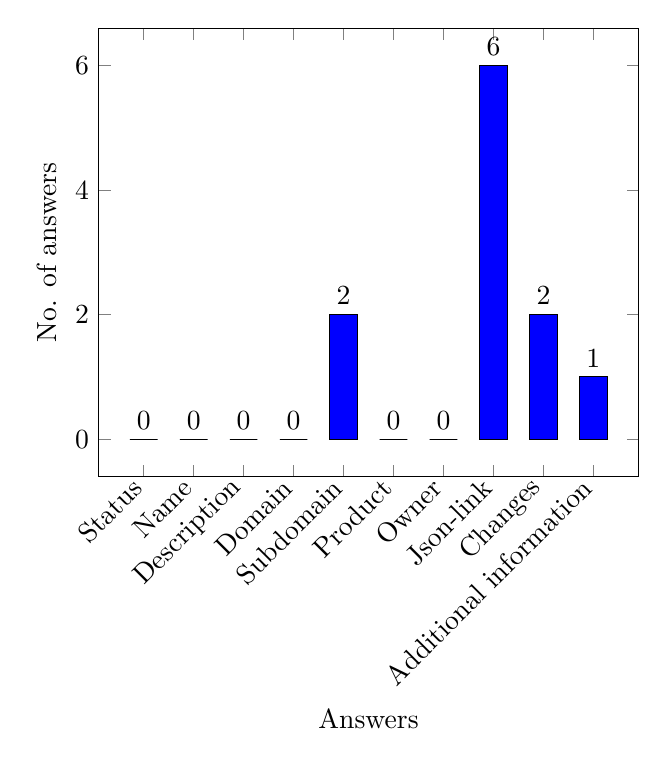
\begin{tikzpicture}
\begin{axis}
[
    %title={Imposing the team to use a predefined toolchain for the application development is easy to establish},
    xtick=data,
    symbolic x coords={Status, Name, Description, Domain, Subdomain, Product, Owner, Json-link, Changes, Additional information},
	ylabel=No. of answers,
	xlabel=Answers,
	x tick label style={rotate=45,anchor=east},
	nodes near coords,
	nodes near coords align={vertical},
]
\addplot 
    [ybar,fill=blue]
	coordinates {(Status,0) (Name,0) (Description,0) (Domain, 0) (Subdomain, 2) (Product, 0) (Owner, 0) (Json-link, 6) (Changes, 2) (Additional information, 1)};
\end{axis}
\end{tikzpicture}
\caption{Question 4.4: The following information displayed in the general section of the detailed view of an application/service is NOT useful}
\label{fig:question44}
\end{figure}

\textbf{Json-link}: 50 percent of the experts considered the json-link as not useful. 
This attribute showed the json-response of the database. It contained every key-value pair stored in the database. This result was expected since enterprise architects and product owners are not interested in every detail of a database entry. Therefore the attribute was removed from the general section.

\textbf{Changes}: EA7 and PO3 replied that the changes of an artifacts regarding the last documentation status and deployment status are not relevant. When the experts were asked what attributes they consider useful EA1 and EA3 did not mark the changes attribute. In question 1.3 more than 80 percent stated that the information in a EA tool is outdated and the rest considered the information as partially outdated. If the experts do not consider the changes as useful how can an enterprise architect determine the state (actual or outdated) of the EA information? This result was not expected.

\subsubsection{Runtime section}

9 experts considered every information as useful. 2 experts marked the instances as useful and everything else as not useful. The running instances of an application running on the cloud is indicates an increase in user load and concurrent requests ergo it is an indicator for the traffic on the application. Therefore 2 experts were only interested in the instances. EA7 was not interested in any of the KPIs shown in this section but expected the running costs to be displayed since the costs are calculated based on the resources consumption. Considering that enterprise architects and product owners demanded costs during the interviews, the running costs of the application was included to this section. The amount of http-calls was also included to this section because it was also demanded during the interviews.

\subsubsection{Metrics monitoring section}

8 of the 12 experts interviewed contemplate the section as useful. 2 experts considered the response time and the url as important. PO2 only considered the response time as valuable and PO1 marked as well the response time as the Prometheus\footnote{\url{https://prometheus.io/}} link (monitoring agent) as relevant.

\subsubsection{Services section}

11 experts see this section as useful since it shows the communication to other services running in the cloud environment. Only 1 of the experts did not give any statements regarding the usage of this section.

\subsubsection{Software dependencies section}

All of the experts stated that this section is important due to several reasons:
\begin{itemize}
    \item Indicator for the complexity of the software
    \item Indicator for dependencies to third party software
    \item Management of software frameworks and technologies throughout the whole enterprise
    \item Detection of outdated components
\end{itemize}
This results were not expected from the enterprise architects since enterprise architects are mostly interested in a holistic view of the IT landscape. As well enterprise architects as product owners pointed this section as crucial.

\subsubsection{Jira monitoring section}
The opinions about the usage of the Jira monitoring section were different. Figure~\ref{fig:question414} shows the different answers. The reason why "project progress" was not very often perceived as useful is that there was no added value since the total issues and open issues were already displayed. More information about the individual issues were required such as links or status of the issues. Depending on the size of the project the visualization of individual issue information can result in an enormous amount of information just in this section.
\begin{figure}[htpb]
\centering
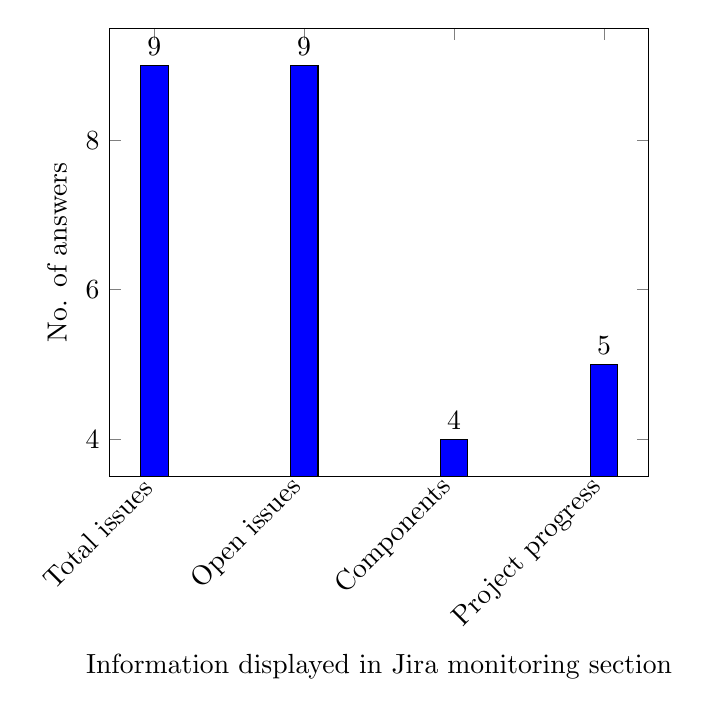
\begin{tikzpicture}
\begin{axis}
[
    xtick=data,
    symbolic x coords={Total issues, Open issues, Components, Project progress},
	ylabel=No. of answers,
	xlabel=Information displayed in Jira monitoring section,
	x tick label style={rotate=45,anchor=east},
	nodes near coords,
	nodes near coords align={vertical},
]
\addplot 
    [ybar,fill=blue]
	coordinates {(Total issues, 9) (Open issues,9) (Components,4) (Project progress, 5)};
\end{axis}
\end{tikzpicture}
\caption{Question 4.14: The following information in the Jira monitoring section is useful}
\label{fig:question414}
\end{figure}

\subsubsection{Github monitoring section}

3 the interviewed experts regard the display of the contributors as delicate due to compliance reasons. 2 of the industry partners did not see the "lines of code" as a valuable indicator. The static analysis of code quality and continuous inspection to perform automatic reviews was named several times. Other metrics mentioned were information on programming languages, cyclomatic complexity and more complex indicators.
% More static code analysis
% Information on programming languages
% More metrics e.g. cyclomatic complexity

\subsubsection{Jenkins section}

More than half of the interviewed experts replied that all metrics displayed in the Jenkins section are relevant. The result of the last job and the duration were the most ticked answers.

\subsubsection{Visualizations section}
The presented visualizations of the tool were perceived as useful. EA5 mentioned that an additional cluster diagram would be useful as well. PO1 also mentioned a pie chart as an additional visualization. Both requirements are justified but the main idea of the tool is to export the data to the EA tool in place for additional visualizations. 

\subsubsection{Additional requirements}\label{subsubsection:additionalrequirementsazd}
During the evaluation additional requirements for the tool were named. The evaluation questionnaire was extended some the questions regarding the requirements. Table~\ref{tab:additionalcasestudyrequirements} lists the additional requirements.

\begin{table}[htpb]
  \caption[Automated EAD requirements derived from the case study]{Automated EAD requirements derived the case study}\label{tab:additionalcasestudyrequirements}
  \centering
  \begin{tabular}{l l l}
    \toprule
      Id & Requirement\\
    \midrule
      AR1 & Business Impact Analysis of applications\\
      AR2 & Data privacy compliance\\
      AR3 & Automated verification of the 12 factor app\\
      AR4 & Automated verification of a resilience pattern\\
      AR5 & Integration of the architecture belt\\
      AR6 & Additional KPIs\\
    \bottomrule
  \end{tabular}
\end{table}

\textbf{AR1}: A Business Impact Analysis of applications is not only required by the enterprise, it is also required due to regulations. The enterprise can analyze in case of a sinister what applications are affected and which related systems are implied by a failure. It can quantify the economic impact of failures.

\textbf{AR2}: Tools have to be compliant with the data privacy regulation. An enterprise needs to know what applications store personal data. 

\textbf{AR3}: The presented approach and tool enables an automated EAD of cloud applications. Therefore a static analysis of the code quality regarding the suitability for deployment on cloud platforms was required. The required methodology for verifying this suitability is the 12 factor methodology\footnote{\url{https://12factor.net/}}. 90 percent of the experts declared that this methodology would indicate if the application is cloud-ready or not (question 4.22).

Due to time constraints a fully implementation of the 12 factor app criteria was not possible. The following paragraphs show the status of the implemented criteria. An improved implementation is seen as valuable for future implementations.
\begin{itemize}
\item \textbf{I. Codebase:} Is the artifact linked to a repository? Since the build and deployment pipeline is only possible if a repository is linked the CD tool this criteria is always fulfilled. 

\item \textbf{II. Dependencies:} Configuration files are searched within the repository. The configuration files should declare software-dependencies, if this is not the case, this criteria is not fulfilled.

\item \textbf{III. Config:} This criteria is fulfilled if configuration files are found. Depending on the programming language or framework specific configurations files are predetermined. The search of the configuration files depends on that. Example configuration files are yaml-files, application.properties, package.json, etc.

\item \textbf{IV. Backing Services:} In some cloud environments the backend services are attached to an artifact. In Cloudfoundry, the specific environment used for this work, the attached services can be queried. If an attached services is a database the criteria is fulfilled. 

\item \textbf{V. Build, release, run:} Version numbers and release numbers are search within the repository. This search does not accord the specification of the criteria but there is no standard process for versioning and release management in the evaluated enterprise. The search for a version number or a release number was considered useful.

\item \textbf{VI. Processes:} Cloudfoundry is used as the cloud infrastructure. This environment does not allow that the the app is executed as one or more processes. Therefore this criteria is always fulfilled. 

\item \textbf{VII. Port binding:} The declaration of static ports within the code is not allowed. A text search was implemented to very this criteria. If static ports are declared within the code, this criteria is not fulfilled.

\item \textbf{VIII. Concurrency:} Not implemented.

\item \textbf{IX. Disposability:} Not implemented.

\item \textbf{X. Dev/prod parity:} The configuration files for the development, staging, and production environment are searched within the repository. These files should be as similar as possible. Depending on the programming language there are some conventions for the specification of these files. For example, in the case of Springboot applications, the configurations files are usually stored with the prefix "dev" and "prod". If the files are found, the similarity has to be compared. A text similarity can be implement for the comparison. The comparison of the attached services or tools has not been implemented.

\item \textbf{XI. Logs:} This criteria is fulfilled if the artifact does not use log dependencies.

\item \textbf{XII. Admin processes:} Not implemented.
\end{itemize}

\textbf{AR4}: Due to a connection to the code repository of the developed artifact a continuous inspection is enabled. The code quality can be automatically reviewed with static code analysis. Therefore enterprise architects required an integration of the following criteria defined by the resilience pattern of the studied enterprise:
\begin{itemize}
    \item Is the application running on the enterprise cloud?
    \item Redundancy checks
    \item Zero downtime deployment verification
    \item Retry verification
    \item Isolation verification
    \item Caching verification
    \item Fallback verification
    \item Loose coupling degree calculation
\end{itemize}
All answers of question 4.23 affirm that an automated test of the resilience pattern is helpful to determine the elasticity of an application.

\textbf{AR5}: The architecture belt is a web application that enables and support the a collaborative approach to establish architecture principles and guidelines. The product owners expressed during the interviews that it is challenging for the team to follow architecture guidelines because these are not well transmitted by the enterprise architects. All experts of the case study asserted that a combination with this tool would also display the overall status of an application regarding the compliance with the architecture guidelines.

Figure~\ref{fig:governance-monitoring-section} shows an additional section implemented due to \textbf{AR3}, \textbf{AR4} and \textbf{AR5}.
\begin{figure}[htpb]
  \centering
  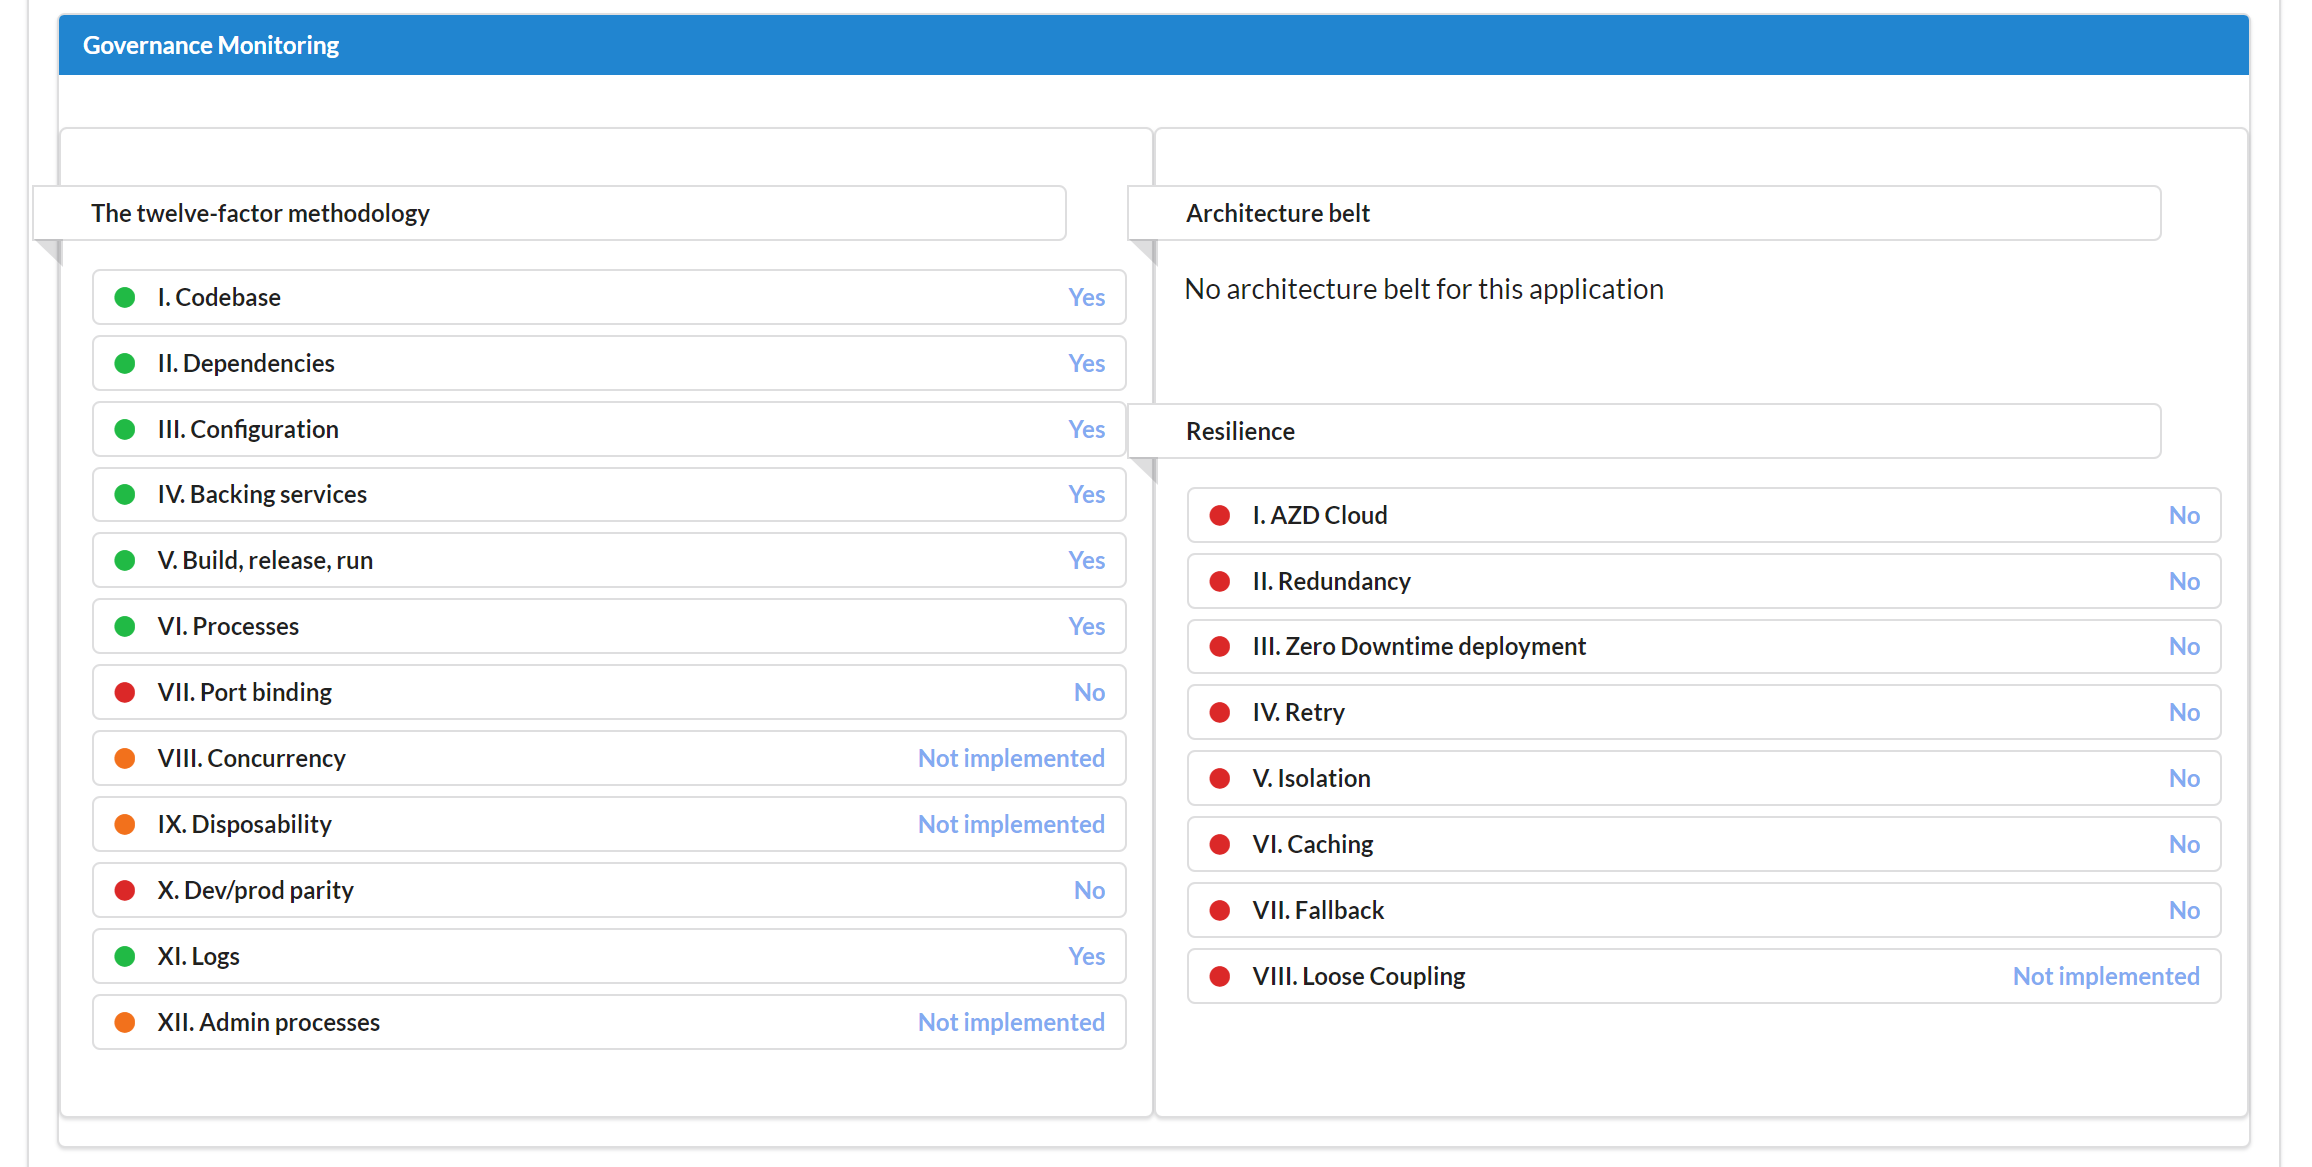
\includegraphics[width=1.0\textwidth]{figures/pivio-detailview-governance-monitoring.PNG}
  \caption{Additional implemented section: Governance monitoring section}
  \label{fig:governance-monitoring-section}
\end{figure}

%TCO, MTBF, Users on app in realtime, Costs, MTTR, MTTF
\textbf{AR6}: Additional KPIs were mentioned during the interviews. Some of the most mentioned KPIs are: Total costs of ownership, mean time between failures, mean time to repair, mean time to failure and real time data of users on the individual applications such as average time per user on app, individual API calls, etc.

\subsection{Evaluation summary}

%5.1 process automates EAD for clouds: 3 strongly agree, 9 agree
As mentioned before 100 percent of the interviewed industry partners stated that the presented process automates the EA documentation of the artifacts running a cloud infrastructure (question 5.1). 

%4.1 views for different stakeholder: 3 Strongly 8 agree 1 disagree
Regarding the presented tool the opinions about the different sections were not always aligned. The sections cover different information for different stakeholder. This statement was supported by question 4.1. Over 90 percent of the experts confirmed this. 

%5.2 overall score: 10 x 4, 2 x 5 = 4,17
The experts were asked to value the approach in combination with the tool. The overall score 4.17 was achieved.





